\documentclass[a4paper,12pt]{article}
\usepackage[top = 2.5cm, bottom = 2.5cm, left = 2.5cm, right = 2.5cm]{geometry}
\usepackage[T1]{fontenc}
\usepackage[utf8]{inputenc}
\usepackage{multirow} 
\usepackage{booktabs} 
\usepackage{graphicx}
\usepackage[spanish]{babel}
\usepackage{setspace}
\setlength{\parindent}{0in}
\usepackage{float}
\usepackage{fancyhdr}
\usepackage{amsmath}
\usepackage{amssymb}
\usepackage{amsthm}
\usepackage[numbers]{natbib}
\newcommand\Mycite[1]{%
	\citeauthor{#1}~[\citeyear{#1}]}
\usepackage{graphicx}
\usepackage{subcaption}
\usepackage{booktabs}
\usepackage{etoolbox}
\usepackage{minibox}
\usepackage{hyperref}
\usepackage{xcolor}
\usepackage[skins]{tcolorbox}
%---------------------------

\newtcolorbox{cajita}[1][]{
	 #1
}

\newenvironment{sol}
{\renewcommand\qedsymbol{$\square$}\begin{proof}[\textbf{Solución.}]}
	{\end{proof}}

\newenvironment{dem}
{\renewcommand\qedsymbol{$\blacksquare$}\begin{proof}[\textbf{Demostración.}]}
	{\end{proof}}

\newtheorem{problema}{Problema}
\newtheorem{definicion}{Definición}
\newtheorem{ejemplo}{Ejemplo}
\newtheorem{teorema}{Teorema}
\newtheorem{corolario}{Corolario}[teorema]
\newtheorem{lema}[teorema]{Lema}
\newtheorem{prop}{Proposición}
\newtheorem*{nota}{\textbf{NOTA}}
\renewcommand\qedsymbol{$\blacksquare$}
\usepackage{svg}
\usepackage{tikz}
\usepackage[framemethod=default]{mdframed}
\global\mdfdefinestyle{exampledefault}{%
linecolor=lightgray,linewidth=1pt,%
leftmargin=1cm,rightmargin=1cm,
}




\newenvironment{noter}[1]{%
\mdfsetup{%
frametitle={\tikz\node[fill=white,rectangle,inner sep=0pt,outer sep=0pt]{#1};},
frametitleaboveskip=-0.5\ht\strutbox,
frametitlealignment=\raggedright
}%
\begin{mdframed}[style=exampledefault]
}{\end{mdframed}}
\newcommand{\linea}{\noindent\rule{\textwidth}{3pt}}
\newcommand{\linita}{\noindent\rule{\textwidth}{1pt}}

\AtBeginEnvironment{align}{\setcounter{equation}{0}}
\pagestyle{fancy}

\fancyhf{}









%----------------------------------------------------------
\lhead{\footnotesize Modelación y Simulación}
\rhead{\footnotesize  Rudik Roberto Rompich}
\cfoot{\footnotesize \thepage}


%--------------------------

\begin{document}
 \thispagestyle{empty} 
    \begin{tabular}{p{15.5cm}}
    \begin{tabbing}
    \textbf{Universidad del Valle de Guatemala} \\
    Departamento de Matemática\\
    Licenciatura en Matemática Aplicada\\\\
   \textbf{Estudiante:} Rudik Roberto Rompich\\
   \textbf{Correo:}  \href{mailto:rom19857@uvg.edu.gt}{rom19857@uvg.edu.gt}\\
   \textbf{Carné:} 19857
    \end{tabbing}
    \begin{center}
        CC3039 - Modelación y Simulación - Catedrático: Oseas Paredes\\
        \today
    \end{center}\\
    \hline
    \\
    \end{tabular} 
    \vspace*{0.3cm} 
    \begin{center} 
    {\Large \bf Microproyecto 1
} 
        \vspace{2mm}
    \end{center}
    \vspace{0.4cm}
%--------------------------

\begin{problema}
	Considere el siguiente proceso de Markov. La gerencia de la \textit{New Fungled Softdrink Company} cree que la probabilidad de que
	un cliente que compra Red Pop o la competencia más importante de la empresa, Súper Cola, está basada en la compra más
	reciente del cliente. Suponga que las siguientes probabilidades de transición son apropiadas:
	\begin{figure}[H]
		\centering
		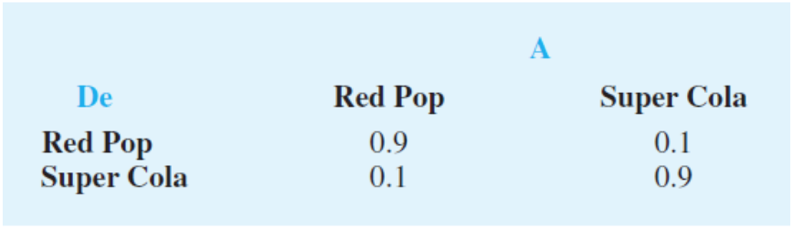
\includegraphics[scale=0.3]{Images/1}
	\end{figure}

\begin{enumerate}
	\item Muestre el diagrama de árbol de dos periodos para un cliente que por última vez compró Red Pop. ¿Cuál es la
	probabilidad de que este cliente compre Red Pop por segunda vez?
	\begin{sol}
		El diagrama de árbol es el siguiente: 
		\begin{figure}[H]
			\centering
			
\includegraphics[scale=0.5]{Images/1.1}
		\end{figure}
	De lo cual tenemos de la primera rama: 
	$$P_1= 0.9\times 0.9=0.81$$
	De la segunda rama: 
	$$P_2=0.1\times 0.1= 0.01$$
	Con lo que podemos concluir: 
	$$P_1+P_2= 0.81+0.01=0.82$$
	Por lo tanto, habrá una probabilidad del 82\% de comprar Red Pop por segunda vez. 
	\end{sol}
	\item ¿Cuál es la cuota de mercado a largo plazo para cada uno de estos productos?
	\begin{sol}
		Se deduce a través de: 
		$$\begin{pmatrix}
			\pi_1 & \pi_2 
		\end{pmatrix} =\begin{pmatrix}
		\pi_1 & \pi_2 
	\end{pmatrix} \cdot \begin{pmatrix}
		0.9 & 0.1\\
		0.1 & 0.9
	\end{pmatrix}$$
De donde se deduce el siguiente sistema de ecuaciones 
$$ \begin{cases}
	\pi_1 = 0.9\pi_1 +0.1 \pi_2\\
	\pi_2 = 0.1 \pi_1+ 0.9\pi_2
\end{cases} \implies \begin{cases}
-0.1\pi_1 +0.1\pi_2&=0\\
0.1\pi_1 -0.1\pi_2 &=0
\end{cases}  $$
En donde $\pi_1+\pi_2=1$, tal que 
$$\begin{cases}
	\pi_1 = 0.5\\
	\pi_2 = 0.5\\
\end{cases}$$
Por lo tanto, la cuota de mercado para cada una es de 50\%. 
	\end{sol}
	\item Se planea una campaña de publicidad para Red Pop, a fin de incrementar la probabilidad de atraer clientes de Super
	Cola. La gerencia cree que la nueva campaña incrementará la probabilidad a 0.15 de que un cliente cambie de Super
	Cola a Red Pop. ¿Cuál es el efecto proyectado de la campaña publicitaria en las cuotas de mercado?
	\begin{sol}
		Se deduce a través de: 
		$$\begin{pmatrix}
			\pi_1 & \pi_2 
		\end{pmatrix} =\begin{pmatrix}
			\pi_1 & \pi_2 
		\end{pmatrix} \cdot \begin{pmatrix}
			0.9 & 0.1\\
			0.15 & 0.85
		\end{pmatrix}$$
		De donde se deduce el siguiente sistema de ecuaciones 
		$$ \begin{cases}
			\pi_1 = 0.9\pi_1 +0.15 \pi_2\\
			\pi_2 = 0.1 \pi_1+ 0.85\pi_2
		\end{cases} \implies \begin{cases}
			-0.1\pi_1 +0.15\pi_2&=0\\
			0.1\pi_1 -0.15\pi_2 &=0
		\end{cases}  $$
		En donde $\pi_1+\pi_2=1$, tal que 
		$$\begin{cases}
			\pi_1 = 0.6\\
			\pi_2 = 0.4\\
		\end{cases}$$
		Por lo tanto, la cuota de mercado para RC es de 60\% y SC es de 40\%.   
	\end{sol}
\end{enumerate}
\end{problema}

\begin{problema}
	Considere el siguiente proceso de Poisson, el cual es más realista ya que le piden que genere un resultado o resultados de simulación con un gran número de ensayos y los utilice para formular conclusiones sobre el comportamiento en estudio. Este problema requiere el uso de una computadora para realizar los cálculos de la simulación.
	El modelo de línea de espera de Burger Dome visto en clase estudia el tiempo de espera de los clientes en su restaurante de comida rápida. El sistema de línea de espera de un solo canal de Burger Dome tiene una tasa de llegadas de $0.75$ clientes por minuto y una tasa de servicio de 1 cliente por minuto.
	
	
	\begin{enumerate}
		\item  Utilice una hoja de trabajo basada en el ejercicio de simulación para un cajero automático para Hammondsport Savings Bank, a fin de simular la operación de esta línea de espera. Suponga que las llegadas de los clientes siguen una distribución de probabilidad de Poisson, los tiempos entre llegadas pueden simularse con la fórmula " $=(-1 / \lambda) *$ LN $(\text { ALEATORIO }())^{\prime \prime}$, donde $\lambda=0.75 .$ Asuma que el tiempo de servicio sigue una distribución de probabilidad exponencial, los tiempos de servicio pueden simularse con la fórmula " $-\mu * L N(\text { ALEATORIO }())^{\prime \prime}$, donde $\mu=1$. Ejecute la simulación con 500 clientes. El modelo analítico indica un tiempo de espera promedio de 3 minutos por cliente. ¿Qué tiempo de espera promedio muestra su modelo de simulación?
		\begin{sol}
			Dada la simulación: 
			\begin{figure}[H]
				\centering
				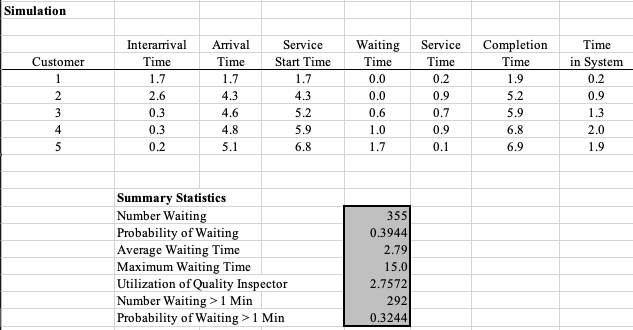
\includegraphics[scale=0.5]{Images/2.1}
				\caption{Plantilla de Quantitative Methods for Business de Anderson et al. }
			\end{figure}
		El tiempo de espera de las 500 simulaciones es de 2.79 minutos; lo cual es lógico, ya que el número de simulaciones es reducido. 
		\end{sol}
		\item Una ventaja de la simulación es que el modelo es fácil de modificar para reflejar otros supuestos sobre los datos de entrada probabilísticos. Suponga que una distribución de probabilidad normal con una media de 1 minuto y una desviación estándar de $0.2$ minutos describe con más precisión el tiempo de servicio. Esta distribución muestra menos variabilidad del tiempo de servicio que la distribución de probabilidad exponencial utilizada en la parte (a). ¿Cuál es el impacto de este cambio en el tiempo de espera promedio?
		\begin{sol}
			Dada la simulación: 
			\begin{figure}[H]
				\centering
				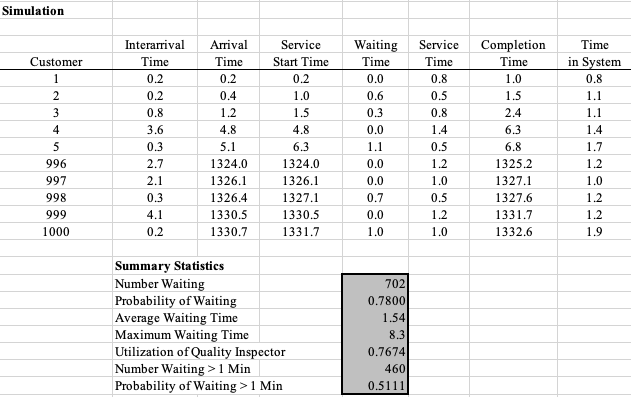
\includegraphics[scale=0.5]{Images/2.2}
				\caption{Plantilla de Quantitative Methods for Business de Anderson et al. }
			\end{figure}
		El tiempo de espera se ve reducido a la mitad aproximadamente. 
		\end{sol}
	\end{enumerate}
	
\end{problema}

\begin{problema}
	Cuando intente el problema siguiente se requerirá que sepa utilizar Excel.
	En el problema de Heidman's Department Store visto en clase, suponga que la siguiente matriz de transición es apropiada:
	$$
	P=\left(\begin{array}{cccc}
		1.0 & 0.0 & 0.0 & 0.0 \\
		0.0 & 1.0 & 0.0 & 0.0 \\
		0.5 & 0.0 & 0.25 & 0.25 \\
		0.5 & 0.2 & 0.05 & 0.25
	\end{array}\right)
	$$
	Si Heidman's tiene $\$ 400$ en la categoría de 0-30 días y \$5000 en la categoría de $31-90$ días, ¿cuál es su estimación de la cantidad de deudas incobrables que la empresa experimentará?
	\begin{sol}
		Considerando la siguiente deducción hecha en \textit{Python}, tenemos: 
		\begin{figure}[H]
			\centering
			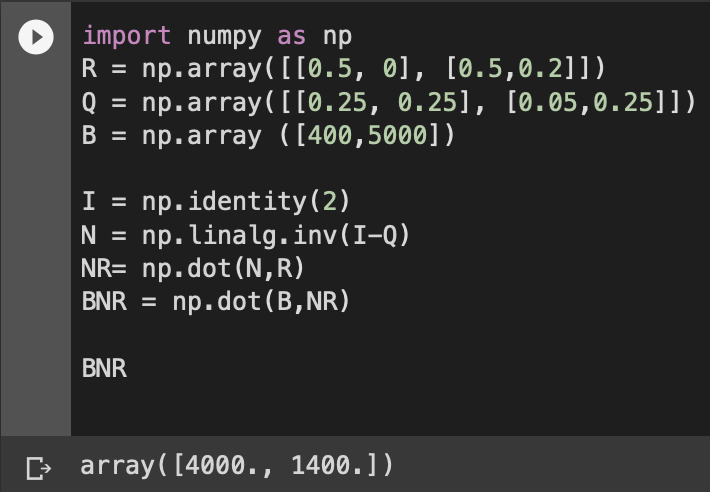
\includegraphics[scale=0.5]{Images/3}
		\end{figure}
	De lo que podemos concluir que las deudas incobrables serán de \$1400. 
	\end{sol}
\end{problema}

%---------------------------
%\bibliographystyle{apa}
%\bibliography{referencias.bib}

\end{document}